% ------------------------------------------------------------------------------
% Este fichero es parte de la plantilla LaTeX para la realización de Proyectos
% Final de Grado, protegido bajo los términos de la licencia GFDL.
% Para más información, la licencia completa viene incluida en el
% fichero fdl-1.3.tex

% Copyright (C) 2012 SPI-FM. Universidad de Cádiz
% ------------------------------------------------------------------------------

%En esta sección se describen todos los aspectos relativos a la gestión del proyecto: metodología, organización, costes, planificación, riesgos y aseguramiento de la calidad.


% \section{\IfLanguageName{english}{Organization}{Organización}}
% \label{section:organizacion}
\begin{comment}
Relación de las personas (roles) involucradas en el proyecto y de cómo se estructuran
las relaciones entre las mismas para ejecutar el proyecto. Relación de los recursos inventariables
utilizados en el proyecto: equipamiento informático (hardware y software), herramientas empleadas, etc. 
\end{comment}

\section{El Centro Aeroespacial Alemán (DLR)}
\label{section:dlr}

\begin{wrapfigure}{r}{0.3\textwidth}
  \begin{center}
    
\includegraphics[width=0.29\textwidth]{dlr-logo.jpg}
  \end{center}
  \caption{Logotipo \gls{dlr}}
\end{wrapfigure}

El \gls{dlr} es una de las instituciones públicas más importantes dedicadas a la investigación en la República Federal Alemana.\\ 

Sus oficinas centrales se encuentran en la ciudad de Colonia, más de 15 delegaciones, con 32 institutos, repartidas por el territorio nacional alemán y 5 situadas a lo largo del mundo \cite{dlrort}. Actualmente cuenta con más de 7.700 trabajadores y un presupuesto anual dependiente del \gls{bmwi}- de 157 millones de euros para el año 2014 \cite{haushalt2014}.\\


En instituciones orientadas a la investigación, como es el \gls{dlr}, la gestión del conocimiento tiene un significado muy importante. Dado el cambio de personal constante involucrado en las distintas fuentes de conocimiento, reside el peligro de pérdida del mismo. \\

La importancia de la gestión del conocimiento es debido a que éste concreta las actividades de una entidad. Estas actividades ``tienen como meta una mejora de la gestión específica de la organización tanto para el conocimiento interno como externo'' \cite{cissek}. Por lo tanto, el objetivo no debería de ser sólo el almacenamiento sino también la recuperación y reutilización del conocimiento obtenido en situaciones anteriores \cite{dengel}.\\


\subsection{``Transporte y la Movilidad'' en el DLR}

Junto con materias relacionadas con la aeronáutica, el espacio, la energía y la seguridad, el transporte es uno de sus temas de estudio, destacando la evolución de éste como unos de los puntos de trabajo más importantes. Tanto es así que 26 institutos del \gls{dlr} contribuyen en su competencia específica a la mejora del ámbito del transporte. La mayoría de ellos generan gran cantidad de conjuntos de datos estadísticos y bases de datos por lo que la gestión del conocimiento juega un papel clave en puntos como el almacenaje, descripción y su (re)utilización. En el campo de investigación sobre el trasporte y sus datos existen actualmente dos portales en el \gls{dlr}; el ``\gls{monitor}'' del \gls{fw}, implementación del \gls{framework}  \gls{kf}, que aporta datos sobre el transporte aéreo y el portal ``\cs'' del \gls{vf} contribuye con los datos sobre la investigación del transporte.


\subsubsection{\fw{}}
El foco de la investigación de este instituto es examinar cómo los dos sistemas, el tráfico aéreo y el sistema de aeropuertos, evolucionan con paso del tiempo bajo ciertas condiciones y cómo conseguir un estado deseado para cada uno. Para ello, el instituto realiza las siguientes tareas:

\begin{itemize}
  \item Analizar la situación y el desarrollo actual.
  \item Examinar la posible evolución futura de ambos sistemas, por ejemplo, a través de estudios de simulaciones.
  \item La construcción de herramientas de software para ayudar a evaluar las condiciones actuales y evitar situaciones indeseables.
  \item Desarrollar métodos para gestionar los aeropuertos de forma eficiente.
  \item Observar los efectos de las medidas aplicadas.
\end{itemize}

Por lo tanto, el objetivo de la investigación del transporte aéreo es el desarrollo de estrategias y medidas destinadas a introducir cambios en la infraestructura o las nuevas regulaciones para el sistema de transporte aéreo en su conjunto a largo plazo.\\

Tiene como objetivo la investigación del sistema aeroportuario en el desarrollo de medidas para gestionar los aeropuertos de manera eficiente. A través del estudio del movimiento de pasajeros en los procesos de la parte pública y los procesos de parte aeronáutica se intenta fomentar un transporte intermodal eficiente \cite{fwHome}.

%Tiene como objetivo la investigación del sistema aeroportuario en el desarrollo de medidas para la gestión en los aeropuertos de manera eficiente el movimiento de pasajeros en los procesos de la parte pública y la parte aeronáutica fomentando de este modo un transporte intermodal eficiente \cite{fwHome}.

\subsubsection{\vf{}}
Este instituto es el principal proveedor oficial para los hogares alemanes de encuestas y estadísticas relacionadas con el transporte. Aporta datos de sobre el trasporte público y encuestas de movilidad.\\ 

Sus investigaciones se centran en los avances y perspectivas del transporte de pasajeros y comercial para conseguir en el futuro un sistema de transporte moderno, eficiente y sostenible para las personas y el medio ambiente.\\ 

Los campos de investigación del instituto son: 
\begin{itemize}
	\item Estudios de patrones de movilidad sobre viajes domésticos y de negocios de personas.
    \item Modelos para representar y prever la demanda de trasporte regional de pasajeros y comercial.
    \item Evaluación de las tecnologías y medidas en cuanto su posible efectividad.
    \item La aceptación y uso efectivo de la red eléctrica para el trasporte de pasajeros y comercial.
    \item Las interacciones entre la información y la comunicación (TIC) con la movilidad.
\end{itemize}

Este instituto está conectado en red a través de la cooperación en investigación y proyectos a nivel nacional e internacional. Colaborando estrechamente con la docencia e investigación universitaria y la enseñanza en centros de educación superiores y de investigación \cite{vfHome}.


Los institutos \gls{vf} y \gls{fw} asignaron como personas responsables de velar por las necesidades de sus institutos, y por lo tanto de la visión proporcionada de su conocimiento por este proyecto, a varios \glspl{reshfellw}. Éstos, coordinados por el \gls{scvss}, colaboraron muy activamente en la ejecución del proyecto, proporcionando la visión de los institutos y el personal investigador que usará en un futuro la aplicación.\\

\subsection{Equipamiento informático}
Las peculiares características del \gls{dlr} ha condicionado a lo largo del proyecto fuertemente la elección de las herramientas informáticas a usar para este proyecto.

\subsubsection{Software}
Partiendo de una lista con el \gls{software} permitido en el \gls{dlr}, se han utilizado los siguientes programas:

\sparagraph{Herramientas para la gestión}
Para controlar el proceso de \gls{software} y la evolución del proyecto se han utilizado principalmente los programas mostrados en la tabla \ref{table:softgest}.

\begin{center}
\begin {table}[H]
\centering
    \begin{tabular}{ | p{3cm}  p{4cm}   p{3cm}   p{5cm} |}
    \hline
    \textbf{Software} & \textbf{Tipo} & \textbf{Versión} & \textbf{Comentario} \\ \hline
    %%%%%%
    Subversion & \Gls{software} para el control de versiones & 1.7 & Utilizado por defecto en el \gls{dlr} para el desarrollo de \gls{software} propio. \\ \hline
    MantisBT & \Gls{bugT} & 1.2 & Utilizado por defecto en el \gls{dlr} para el desarrollo de \gls{software} propio. \\ \hline
    Jenkins & \Gls{swIntcon} & 1.573 & Utilizado por defecto en el \gls{dlr} para el desarrollo de \gls{software} propio. \\ \hline
    \end{tabular}
    \caption{\Gls{software} usado para la gestión}
    \label{table:softgest}
    \end{table}
\end{center}

\sparagraph{Herramientas del entorno de desarrollo}\\
El entorno de programación donde ha implementado el proyecto se ha sustentando de la ayuda de los programas indicados en la tabla \ref{table:softdev}.

\begin{center}
\begin {table}[H]
\centering
    \begin{tabular}{ | p{3cm}  p{4cm}   p{3cm}   p{5cm} |}
    \hline
    \textbf{Software} & \textbf{Tipo} & \textbf{Versión} & \textbf{Comentario} \\ \hline
    %%%%%%
    \Gls{eclipse} & \gls{ide} & Kepler SR2 & Con los \glspl{plugin} para Subversion, MantisBT y Jenkins  \\ \hline
    Maven & Gestión y construcción de proyectos & 3.2.1 & Conjuntamente con el \gls{plugin} para Eclipse \\ \hline
    JRebel & auto-\Gls{deploy} & 5.6.1 & Conjuntamente con el \gls{plugin} para \gls{eclipse} \\ \hline
    \end{tabular}
    \caption{\Gls{software} usado como entorno de desarrollo}
    \label{table:softdev}
  \end{table}
\end{center}

\sparagraph{Herramientas usadas para el desarrollo}
El producto resultado de este proyecto requiere o ha necesitado en alguna de sus etapas de desarrollo el \gls{software} listado en la tabla \ref{table:softdevsw}.

\begin{center}
\begin {table}[H]
\centering
    \begin{tabular}{ | p{3cm}  p{4cm}   p{3cm}   p{5cm} |}
    \hline
    \textbf{Software} & \textbf{Tipo} & \textbf{Versión} & \textbf{Comentario} \\ \hline
    %%%%%%
    \Gls{java} & Lenguaje de programación & 1.7 & Lenguaje conocido ampliamente por \gls{scvss} \\ \hline
    Wiremock & \Gls{framework} para \gls{sw} & 1.18 & \Gls{mocking} web services \\ \hline
    Spring & \Gls{framework} para la web& 4.0.3 & Conjuntamente con el \gls{plugin} para \gls{eclipse} \\ \hline
    Jackson & Librería \Gls{java}& 1.9.13& Libreria para tratar documentos \gls{json} \\ \hline
    SLF4J & Librería \Gls{java}& 1.9.13& Systema de \gls{logging} \\ \hline
    \end{tabular}
    \caption{\Gls{software} usado para desarrollar el programa}
    \label{table:softdevsw}
  \end{table}
\end{center}

\sparagraph{Herramientas usadas para la fase de \gls{testing}}
Para comprobar el correcto funcionamiento y asegurar la calidad del producto final se han utilizado las herramientas de \gls{software} indicadas en la tabla \ref{table:softtest}.

\begin{center}
\begin {table}[H]
\centering
    \begin{tabular}{ | p{3cm}  p{4cm}   p{3cm}   p{5cm} |}
    \hline
    \textbf{Software} & \textbf{Tipo} & \textbf{Versión} & \textbf{Comentario} \\ \hline
    %%%%%%
    Powermock & Librería \Gls{java} & 1.4 & Usado para simular comportamientos en los test \\ \hline
    EasyMock & Librería \Gls{java} & 3.2 & Usado para simular comportamientos en los test \\ \hline
    JUnit & Librería \Gls{java}  & 4.12& Herramienta de \gls{testing}  de \Gls{java} \\ \hline
    \end{tabular}
    \caption{\Gls{software} usado durante la fase de \gls{testing}}
    \label{table:softtest}
  \end{table}
\end{center}

\sparagraph{Herramientas usadas para el \gls{despliegue}}
El \gls{software} de la tabla \ref{table:sofdesp} fue utilizado tanto durante el desarrollo como en el servidor de pruebas donde reside el proyecto para comprobar en todo su conjunto el correcto funcionamiento y como demostración.

\begin{center}
\begin {table}[H]
\centering
    \begin{tabular}{ | p{3cm}  p{4cm}   p{3cm}   p{5cm} |}
    \hline
    \textbf{Software} & \textbf{Tipo} & \textbf{Versión} & \textbf{Comentario} \\ \hline
    %%%%%%
    \gls{liferay} & Portal de gestión de contenidos & 6.2.1 CE GA2 & Utilizado junto sus \glspl{plugin} para \gls{eclipse} durante el desarrollo \\ \hline
    \gls{tomcat} & Servidor web & 7 &  Usado conjuntamente con gls{liferay} \\
    \hline
    \gls{solr} & \Gls{motorbusqueda}& 4.8.1& \Gls{motorbusqueda} desarrollado en \Gls{java}\\ \hline
    \gls{jetty} & Servidor web & 7& Usado conjuntamente con \gls{solr} \\ \hline
    \end{tabular}
    \caption{\Gls{software} usado para el \gls{despliegue} de la aplicación}
    \label{table:sofdesp}
  \end{table}
\end{center}

\sparagraph{Herramientas usadas para documentación}
Para generar la presente documentación se han utilizado las herramientas expuestas en la tabla \ref{table:softdoc}.

\begin{center}
\begin {table}[H]
\centering
    \begin{tabular}{ | p{3cm}  p{4cm}   p{3cm}   p{5cm} |}
    \hline
    \textbf{Software} & \textbf{Tipo} & \textbf{Versión} & \textbf{Comentario} \\ \hline
    %%%%%%
    write\LaTeX{} & Editor online &  & Editor web para \gls{latex} \\ \hline
    GanttProject & Editor de gráficos & 2.5& Herramienta para la generación de gráficos de \Gls{gantt} \\ \hline
    Gimp & Editor de imágenes &  2.8.10 & Edición de imágenes muy completo \\ \hline
    ConceptDraw & Editor de gráficos &  10  & Edición de gráficos \gls{uml} \\ \hline
    \end{tabular}
    \caption{\Gls{software} usado para la generación de la documentación}
    \label{table:softdoc}
  \end{table}
\end{center}


\sparagraph{Herramientas usadas para la comunicación y coordinación}
Dado el carácter distribuido y descentralizado de los departamentos en el \gls{dlr} y la distancia física que separan cada uno de los agentes implicados en el proyecto, las herramientas de comunicación usadas son un factor clave durante el desarrollo del proyecto, tabla \ref{table:softcomu}.

\begin{center}
\begin {table}[H]
\centering
    \begin{tabular}{ | p{3cm}  p{4cm}   p{3cm}   p{5cm} |}
    \hline
    \textbf{Software} & \textbf{Tipo} & \textbf{Versión} & \textbf{Comentario} \\ \hline
    %%%%%%
    Lync & Servicio de \gls{mensinst} & 4.0.7 & Usado en \gls{dlr} como sistema oficial de comunicación entre los trabajadores \\ \hline
    Outlook & Organizador personal & 14.0.7& Usado en \gls{dlr} como sistema de correo y calendario\\ \hline
    Confluence & \Gls{wiki} & 5.5& \Gls{wiki} para alojar la documentación de los proyectos desarrollados en \gls{dlr} \\ \hline
    \end{tabular}
    \caption{Herramientas usadas para la comunicación y coordinación}
    \label{table:softcomu}
  \end{table}
\end{center}

\subsubsection{\Gls{hardware}}
En lo referente al \gls{hardware}, se distinguen dos máquinas únicamente; la dedicada a la implementación del producto y un servidor usado como máquina de pruebas.

\sparagraph{\Gls{hardware} para el desarrollo}
A continuación se muestra en el cuadro \ref{table:harddev} la información del \gls{hardware} utilizado para el desarrollo del proyecto.


\begin{center}
\begin {table}[H]
\centering
    \begin{tabular}{ | r | r |}
    \hline
    S.O.& Windows 7 \\ \hline
    Procesador & Intel Core 2 Duo P8600 - 2.4GHz \\ \hline
    Memoria RAM & 4 GB \\ \hline
    Pantalla & 15.4" + 22" \\ \hline
    Disco Duro & 500GB \\ \hline
    Tarjeta Gráfica & Intel Graphics Media Accelerator (GMA) 4500MHD \\ \hline
    \end{tabular}
    \caption{\Gls{hardware} del equipo usado para el desarrollo}
    \label{table:harddev}
  \end{table}
\end{center}


\sparagraph{\Gls{hardware} del servidor}
Las propiedades del servidor gestionado por \gls{dlr} donde reside la aplicación de prueba se muestran en la tabla \ref{table:hardserv}.

\begin{center}
\begin {table}[H]
\centering
    \begin{tabular}{ | r | r |}
    \hline
    S.O.& Ubuntu 12.04.04 TLS \\ \hline
    Procesador & Intel® Xeon® Processor E5-2660 \\ \hline
    Memoria RAM & 4 GB \\ \hline
    Disco Duro & 500GB \\ \hline
    \end{tabular}
	\caption{\Gls{hardware} del servidor para la aplicación de pruebas}
    \label{table:hardserv}
  \end{table}
\end{center}

\section{\IfLanguageName{english}{Development Methodology}{Metodología de desarrollo}}

\begin{comment}Definición del proceso de desarrollo, ciclo de vida y metodología empleada durante la elaboración del proyecto. Las fases y/o iteraciones que proponga el método empleado deberán quedar recogidas en la planificación que se detalle más adelante.
\end{comment}

Las fases iniciales del proyecto pueden dividir en los siguientes puntos:

\begin{itemize}
\sitem{Estudio del proyecto \gls{kf}}
La primera fase del proyecto consistió en un estudio exhaustivo de la documentación y la implementación del proyecto predecesor. También se produjeron varias reuniones con los miembros del \gls{scvss} para perfilar los aspectos menos nítidos y confusos del funcionamiento e implementación de \gls{kf}.

\sitem {Estudio de las nuevas necesidades de visualización}
Una vez estudiado y comprendido la situación de la que se partía, se estudiaron las distintas posibilidades de visualización y de interacciones de los usuarios sobre los datos. Todo esto teniendo siempre presente la \gls{ux} como punto clave del estudio. 
% \question{alargar el punto para explicar más? en requisitos? toma de decisiones?}

\sitem{Estudio de las tecnologías disponibles para la visualización}
Para comprobar qué tecnologías son las más apropiadas para obtener una visualización acorde a las necesidades del proyecto y del usuario, se estudiaron un amplio conjunto de tecnologías y opciones de aplicación.\\ 
% \question{alargar el punto para explicar más? en requisitos? toma de decisiones?}
% \todo{alargar punto para incluir las entrevistas y el proceso de estudio con anexo}

\sitem{Estudio de la capa de servicios}
Durante los estudios previos explicados anteriormente, se detectaron grandes dificultades para cubrir los objetivos del proyecto (ver capítulo  \ref{chapter:requisitos}). Esto condicionó que una parte de la aplicación, la implementación capa de servicios, tuviera que replantearse 
%\todo{explicarlo mejor\\ en otra parte\\ del documento\\ o aquí en un\\ apartad} 
en conformidad con la gestión de proyectos en el \gls{scvss} y las necesidades de los institutos \gls{fw} y \gls{vf}.

\end{itemize}

Una vez obtenida toda la información necesaria para el planteamiento del proyecto, se optó por un proceso de desarrollo basado en \glspl{prototipo}, en concreto ``\gls{extreprot}'' \cite{extrPro}\cite{extreprobook} dada su adaptabilidad a las posibles diferentes decisiones a tomar.

\subsubsection{Aplicando ``\gls{extreprot}''}
\label{subsubsection:aplicandoextre}
El ``\gls{extreprot}'' es un proceso para desarrollar aplicaciones, especialmente aplicaciones web, basada en el diseño de \glspl{prototipo} funcionales cada vez más complejos. Este proceso se divide en cuatro fases: 
% \todo{incluir estos pasos para comparar en las conclusiones cuanto tiempo se ha gastad de más}
\begin{itemize}
\sitem{Static Prototype phase} La primera fase consiste en un \gls{prototipo} estático, implementado normalmente \gls{html}. En el caso de este proyecto se optó por bocetos en soporte físico con ejemplos reales implementados en \gls  {html} y \gls{js} para ilustrar a su vez las posibilidades de interacción de los usuarios y comportamiento del producto futuro.

\sitem{Extended Static Prototype phase} En siguiente fase de \gls{extreprot}  se define el modelo lógico de los datos. Los datos provienes de la capa de servicio son definidos. Para el proyecto \gls{kf2} se definió los valores para el índice de búsqueda.

\sitem{Extreme Prototype phase} La tercera fase se apoya la implementación de un \gls{prototipo} dinámico usando el \gls{framework} de programación deseado. Este \gls{prototipo} es totalmente funcional sustentando su funcionamiento en una capa de servicios simulada. Al concluir esta fase, la \gls{ui} quedó definida y su futuro funcionamiento demostrable. 
% \question{Explicar Wiremock? o como se simulo los servicios?}

\sitem{Service Implementation Phase} La última fase del \gls{extreprot}  consiste en la implementación de los servicios anteriormente simulados. Junto con el \gls{prototipo} de la fase anterior y algunos cambios de adaptación se consiguió la integración de todos los componentes implementados anteriormente. 
%\question{Explicar la implementación de los servicios?}
\end{itemize}

En la imagen \ref{image:extreprot} se expone los fundamentos de esta metodología.\\

\begin{figure}[h!]
  \centering
     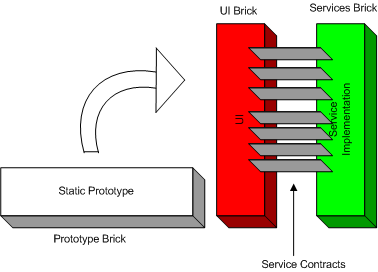
\includegraphics[width=0.6\textwidth]{extreme-prototyping-3-bricks.png}
  \caption{Los tres ``bricks'' o \glspl{prototipo} de \gls{extreprot} \cite{extrPro}}
  \label{image:extreprot}
\end{figure}

Como fase final del presente proyecto se realizaron algunos cambios simples a petición de los institutos \gls{vf} y \gls{fw}. Estos cambios para sirvieron  para precisar el producto obtenido en las anteriores fases. De esta forma, el producto obtenido final a través del \gls{extreprot} cumplió satisfactoriamente las  necesidades planteadas.

\section{\IfLanguageName{english}{Project's Schedule}{Planificación del
proyecto}} 
La planificación inicial del proyecto se puede observar en el diagrama de \gls{gantt} \ref{image:ganttinicial}. En ella se pueden diferenciar la planificación inicial para las distintas fases del desarrollo.\\

No obstante, durante la decisión de la visualización se acordó junto con el \gls{scvss} una replanificación del proyecto alargando su fases de desarrollo y la duración del conjunto del proyecto. Estas modificaciones se observan el la gráfica de \gls{gantt} \ref{image:ganttrepla}.

\begin{comment}
\todo[inline]{Estimación temporal y definición del calendario básico (hitos principales e iteraciones). Desarrollo de la planificación detallada, utilizando un diagrama de Gantt. Los diagramas de Gantt que se vean correctamente (girados y divididos si hace falta).}

En la imagen \ref{image:gantt} se muestra las fases del proyecto temporalmente ordenadas y las relaciones de dependencia entre ellas.
\end{comment}

\begin{figure}
\centering
\begin{minipage}{.5\textwidth}
  \centering
     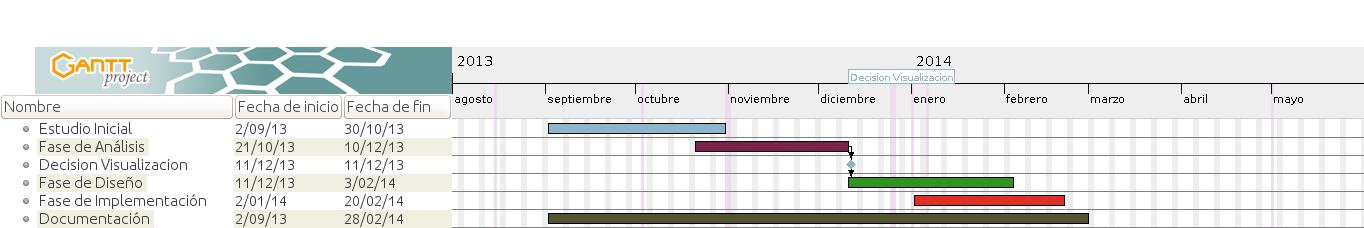
\includegraphics[width=2.5\textwidth, angle=90]{gantt-inicial.png}
  \captionof{figure}{Gráfica inicial de Gantt}
  \label{image:ganttinicial}
\end{minipage}%
\begin{minipage}{.5\textwidth}
  \centering
     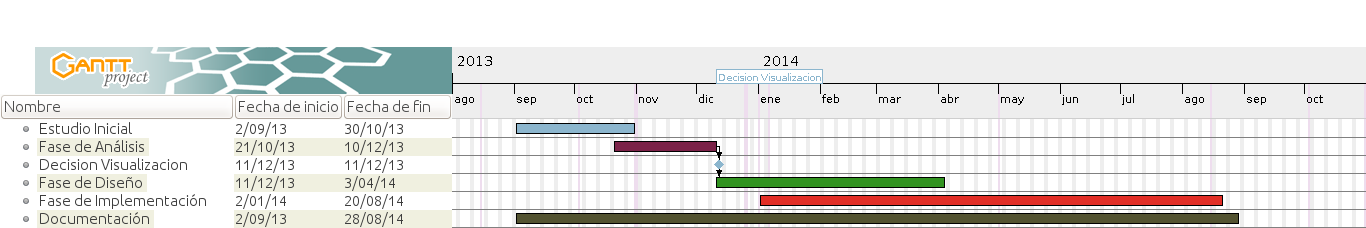
\includegraphics[width=2.5\textwidth, angle=90]{gantt-replanteamiento.png}
  \captionof{figure}{Gráfica de Gantt de la replanificación}
  \label{image:ganttrepla}
\end{minipage}
\end{figure}

%\todo[inline]{
% Se debe incluir una comparación cuantitativa del tiempo y el esfuerzo realmente invertido frente al estimado y planificado. Estos datos pueden recogerse del sistema de gestión de tareas empleado para el seguimiento del proyecto.}\question{cómo hacer la comparación cuantitativa??}

\section{\IfLanguageName{english}{Cost Estimation}{Costes}}
Los costes de este proyecto son principalmente coste de personal. Esto abarca tanto el coste proporcional al salario de cada trabajador del \gls{dlr} que interviene durante el proceso (\gls{vf}, \gls{fw}, \gls{scvss}, personal administrativo del \gls{dlr}, \dots) como los gastos derivados de las reuniones realizas para su realización (dietas, viajes, \dots).\\

Además habría que incluir el uso de las infraestructuras y recursos tecnológicos (\gls{hardware} y \gls{software}) necesitados.\\

Lamentablemente, dada la naturaleza del \gls{dlr}, esta información no puede ser publicada al igual que el presupuesto de partida para este proyecto. En cambio podremos realizar una estimación del coste del proyecto teniendo en cuenta los anteriores factores.\\

\subsection{Estimación}

Si suponemos que el equipo utilizado tiene un coste de 1512\euro{} para un periodo de amortización de tres años se tiene que el coste por mes usado es de 42\euro{}. El mobiliario utilizado y el servidor junto con la infraestructura pertenecen al \gls{dlr} pero implica también tenga un coste relacionado al proyecto, suponemos que asciende a 300\euro{} al mes junto con otros gastos relacionados con el mobiliario (luz, agua, \dots) .\\


El proyecto tiene una estimación temporal de once meses, suponiendo que el desarrollador dedica unas 20 horas semanales, hasta la finalización del proyecto, hace un total de 880 horas (11 meses a 4 semanas por mes). Para las reuniones se estima que se necesitan 40 horas para todos \glspl{reshfellw} y 20 horas de personal administrativo (tabla \ref{table:salmes}).\\

\begin{center}
\begin {table}[H]
    \begin{tabular}{ | l | c | p{6.5cm} |}
    \hline
    \textbf{Cargo} & \textbf{Coste} & \textbf{Descripción} \\
    				& (persona/mes) &                      \\ \hline
    Desarrollador & 5.5 persona/mes & Desarrollador sin experiencia (realiza el producto)\\ \hline
    \gls{reshfellw} & 0,25 persona/mes& Colabora activamente \\ \hline
    Personal administrativo  & 0,125 persona/mes& Gestión de personal y proyectos \\ \hline
    \end{tabular}
    \caption{Resumen del gasto de personal}
    \label{table:salmes}
  \end{table}
\end{center}

Los salarios del personal del \gls{dlr} es público al ser una institución dependiente del Estado. Por lo tanto, partiendo de la tabla de salarios públicos \cite{tvod} obtenemos los datos relevantes para la estimación resumidos en la tabla \ref{table:resucost}. También se destina una partida de 2000\euro{} para reuniones y gastos variados.\\

De forma complementaria, en la tabla \ref{table:resucost} también se muestran los cálculos con los salarios medios obtenidos de la herramienta on-line de Infojobs \cite{infojobs}.\\

Calculando la estimación de todos las variables anteriormente expuestas se obtiene una estimación de 23647,88\euro{}  (13963,94\euro{} en España ).

\begin{center}
\begin {table}[H]
    \begin{tabular}{ |l|c|c|c|c|c|}
    \hline
    \textbf{Recurso} & \textbf{Número de } & \textbf{Precio/unidad } & \textbf{Precio/unidad } & \textbf{Total} & \textbf{Total} \\ 
      & unidades & Alemania(\euro{}) & España(\euro{}) & Alemania(\euro{}) & España(\euro{})\\ \hline
    %%%%%%%
    Desarrollador & 5,5 & 2.965 & 1351,75 & 16307,5 & 7434,625 \\ \hline
    \gls{reshfellw} & 0.25 & 4.558 & 2.254,08 & 1139,5 & 563,5\\ \hline
    Admon. & 0,125 & 3.519 & 1.630,5 & 439,875 & 203,8125\\ \hline
    Equipo & 11 & 42\euro{} & 42\euro{} & 462 & 462 \\ \hline
    Infraestructura & 11 & 300 & 300 & 3300 & 3300 \\ \hline
    Variados & 1 & 2000 & 2000 & 2000& 2000 \\ \hline\hline
    TOTAL &&&& 23647,88 & 13963,94 \\ \hline
    \end{tabular}
    \caption{Resumen de la estimación de los costes}
    \label{table:resucost}
  \end{table}
\end{center}




% \review{Cuenta los costes no reales que estimarías si el proyecto se hiciera en España, incluyendo costes de amortización de equipos y costes de personal según alguna tabla salarial estándar (de la UCA, de infojobs, etc.)}

\begin{comment}
\question{qué puedo poner? algo más?}
\todo[inline]{
Estudio y presupuesto de los costes de los recursos (humanos y materiales) descritos anteriormente, necesarios para el proyecto.

Para el cálculo de costes de personal pueden consultarse las tablas salariales de la UCA para el personal técnico de apoyo contratado laboral \cite{makebst}, o bien otras más ajustadas a la realidad. El cálculo del coste del personal del proyecto debe hacerse en personas-mes, y luego hacer la correspondencia al coste monetario.\\
}
\end{comment}
\section{\IfLanguageName{english}{Risks Estimation}{Riesgos}}
%Enumeración de los riesgos del proyecto, indicando su posible impacto (efecto que la ocurrencia del citado riesgo tendría en el desarrollo del proyecto) y la probabilidad de ocurrencia. Una vez los riesgos son identificados y priorizados, hay que definir los planes necesarios para reducir los efectos del riesgo una vez se haya materializado o disminuir que este ocurra.

En todo proyecto \gls{software} se pueden producir situaciones que difcultarían el proceso de desarrollo, el cumplimiento de los plazos establecidos o desajustarían el presupuesto asignado. Estos riesgos pueden ser causados por numeroso factores de distinta naturaleza. Por ello es necesario el estudio previo de éstos.\\

Utilizando como base MAGERIT versión 3 \cite{MAGERIT}, se van a describir un conjunto de posibles riesgos genéricos y específicos para el desarrollo del proyecto \gls{kf2}.\\

\subsection{Descripción de Riesgos}
En los siguientes puntos se describen los riesgos junto con su valoración del impacto y probabilidad de ocurrencia usando las tablas \ref{table:valoracion} y \ref{table:probabilidad}.

\begin{center}
\begin {table}[H]
\centering
    \begin{tabular}{ | r | r |}
    \hline
\textbf{Valoración} & \textbf{Descripción}  \\ \hline
MB &  Impacto muy bajo \\ \hline
B & Impacto bajo \\ \hline
M & Impacto medio\\ \hline
A & Impacto alto \\ \hline
MA & Impacto muy alto \\ \hline
    \end{tabular}
	\caption{Tabla valoración impacto de riesgos}
    \label{table:valoracion}
  \end{table}
\end{center}

\begin{center}
\begin {table}[H]
\centering
    \begin{tabular}{ | r | r |}
    \hline
\textbf{Ocurrencia} & \textbf{Descripción} \\ \hline
Muy Frecuente(MF) & A diario \\ \hline
Frecuente(F) & Una vez al mes \\ \hline
Frecuencia Normal(FN) & Una vez al año \\ \hline
Poco Frecuente(PF) & Cada varios Años \\ \hline
    \end{tabular}
	\caption{Tabla probabilidad riesgos}
    \label{table:probabilidad}
  \end{table}
\end{center}


\subsubsection{Riesgos genéricos}
Estos tipos de riesgos son comunes para el desarrollo de todo proyecto software:
\begin{enumerate}[label=\bfseries G\arabic*]
	\sitem{Riesgos de servicios (B-FN)}
    Representan la problemática posible causada por la prestación de servicios internos. 
    \sitem{Pérdida de información y datos (MA-PC)}
    Corrupción o pérdida total de los datos almacenados para el proyecto.
    \sitem{Fallos del \gls{software}(A-FN)}
	Problemas causados por errores o fallos del \gls{software}.
    \sitem{Problemas con el \gls{hardware} (MA-PC)}
    Problemas con los elementos físicos usados (ordenadores, impresoras, \dots).
    \sitem{Problemas de personal (M-F)}
    Indisposición inesperada de alguno de los recursos humanos disponibles relacionados con el proyecto.
    \sitem{Problemas de red (FN-M)}
    Fallo de la conexión de los sistemas de comunicación (teléfono, internet, \dots).
\end{enumerate}

\subsubsection{Riesgos específicos}
Los riesgos particulares del presente proyecto son:

\begin{enumerate}[label=\bfseries E\arabic*]
	\sitem{Cambio del origen de datos (A-FN)}
	Si es necesario obtener los datos desde otro sistema de almacenamiento (base de datos, ficheros \gls{xml}, \dots) habría que modificar el sistema de importación para una correcta obtención de éstos.
    
	\sitem{Cambio en el formato del origen de datos (A-FN)}
    Si se modificara la especificación del formato de los datos obtenidos, habría que modificar el sistema de extracción de los mismos.
    
    \sitem{Variación del sistema de información (A-MF)}
    A lo largo de la vida del proyecto, las necesidades del sistema de información pueden variar.
    
    \sitem{Modificación del funcionamiento de la visualización (A-MF)}
    El sistema de visualización puede cambiar obligando al uso o modificación de nuevos Componentes  visuales.
\end{enumerate}

\subsection{Subsanación de los Riesgos}    
El departamento \gls{scvss} dispone de un servidor con \gls{svn}. Usando este sistema a de control de versiones se subsanarán los riesgos que provocan una pérdida de datos (G2-4). Este servidor reside en las instalaciones de T-Systems con copias de seguridad diariamente programadas.\\

Los posibles problemas causados por los riesgos de personal (G5) implican, sobre todo, el replanteamiento de las reuniones con las personas involucradas del \gls{dlr}. Usando una planificación de reuniones a largo plazo con posibles alternativas se evitan, en su mayoría, la repercusión en el proyecto. Respecto al equipo de desarrollo, éste se compone solamente de una persona por lo que este riesgo queda considerablemente acotado en sus efectos y sus posibles opciones para resarcirlo.\\

Para desagraviar los riesgos específicos de la aplicación (E1-4), durante el proceso de desarrollo se ha de estar en contacto directo con el entorno interesado en el proyecto (\textit{Stackeholders}).

\section{\IfLanguageName{english}{Quality Assurance}{Aseguramiento de calidad}}
% \question{qué puedo poner? SVN, Mantis, wiki, jenkins?? testing??}

\begin{comment}
En esta sección se incluirán las actividades y tareas relacionadas con el aseguramiento de calidad a realizar durante el desarrollo del software. Se incluirán los estándares, prácticas y normas aplicables durante el desarrollo del software.\\

También, deberán recogerse los diferentes tipos de revisiones, verificaciones y validaciones que se van a llevar a cabo, los criterios para la aceptación o rechazo de cada producto y los procedimientos para implementar acciones correctoras o preventivas.
\end{comment}
Para asegurar la calidad del proceso de desarrollo y llevar un control sobre el mismo se debe utilizar el \gls{software} \gls{mantis} en conexión con los \textit{commits} realizados en \gls{svn}. Para ello se obliga a que cada \textit{commit} ejecutado esté relacionado con un ticket o tarea previamente definida en \gls{mantis}.\\

La documentación del proyecto generada debe accesible y verificable por el resto de miembros del \gls{scvss} a través de una \gls{wiki} interna.\\

La calidad del código fuente adquiere una relevancia muy alta para asegurar el mantenimiento del \gls{software}. Para ello, hay que prestar especial atención durante el desarrollo en los siguientes aspectos:

\begin{itemize}
	\item Código claro y estructurado.
    \item Utilización de patrones de diseño.
    \item Utilización de estándares de codificación para \gls{java} \cite{javacode}, \gls{js} \cite{javascriptcode} y \gls{html} \cite{htmlcode}.
    \item Código moderadamente comentado.
    \item Utilización de ficheros de configuración.
\end{itemize} 

A través de \gls{testing} se debe asegurar el correcto funcionamiento de la aplicación en sus aspectos más importantes. Junto con \gls{jenkins}, se debe realizar la integración e inspección continua.




